\documentclass[11pt]{article}\usepackage[a4paper,margin=22mm]{geometry}\usepackage{graphicx,booktabs,hyperref}\begin{document}\title{Body-fitted finite-volume DFG 2D-1 cylinder verification}\maketitle\section{Problem and method}DFG 2D-1, Re=20; parabolic inlet and no-slip circular cylinder in a channel. Conforming Gmsh triangles, conservative linear upwind transport, geometric interpolation and Gauss face-pressure integration are verified using raw fields and independent NumPy equation replay. Strict physical errors are below 3\% only for runs explicitly accepted below. Full problem, software commands, references and limits are in report.md.\section{Results}\begin{tabular}{rrrrl}\toprule Cells & Iterations & $C_D$ & $C_L$ & Accepted\\\midrule 8252 & 33 & 5.79708501 & 0.0484330135 & False \\
8252 & 34 & 5.51625733 & 0.0233518549 & False \\
8252 & 35 & 5.54301346 & 0.0100601062 & False \\
\bottomrule\end{tabular}\section{Computed fields and convergence}\begin{figure}[p]\centering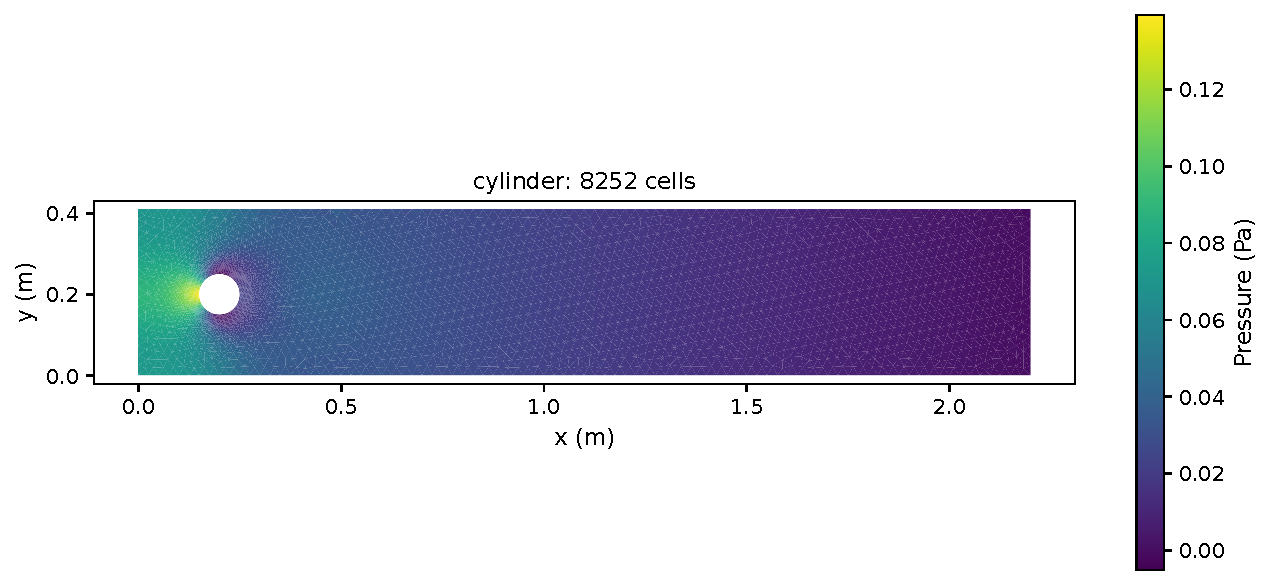
\includegraphics[width=.95\linewidth]{upwind/figures/pressure-global.pdf}\caption{upwind figures pressure global}\end{figure}\begin{figure}[p]\centering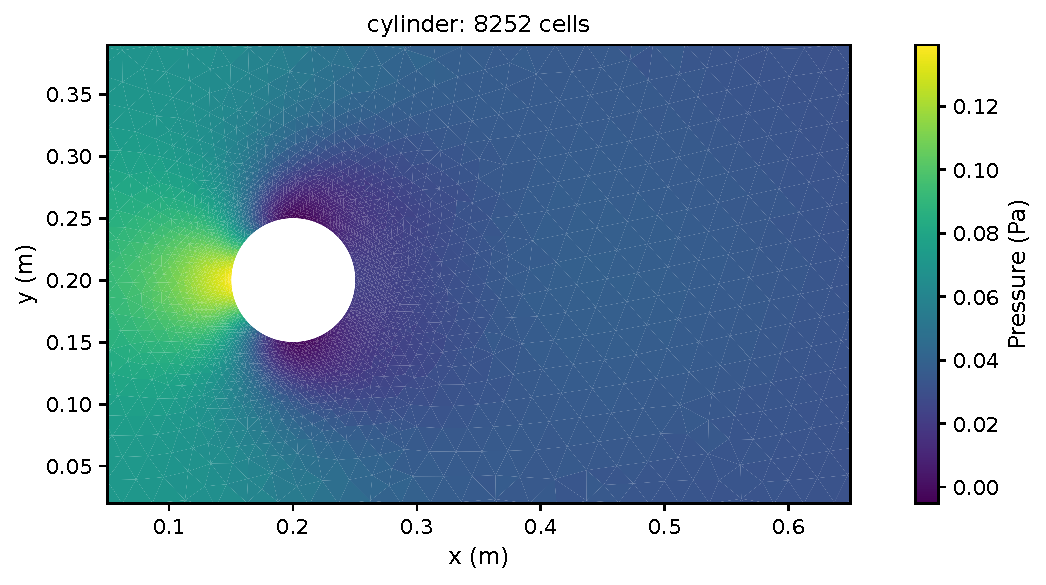
\includegraphics[width=.95\linewidth]{upwind/figures/pressure-local.pdf}\caption{upwind figures pressure local}\end{figure}\begin{figure}[p]\centering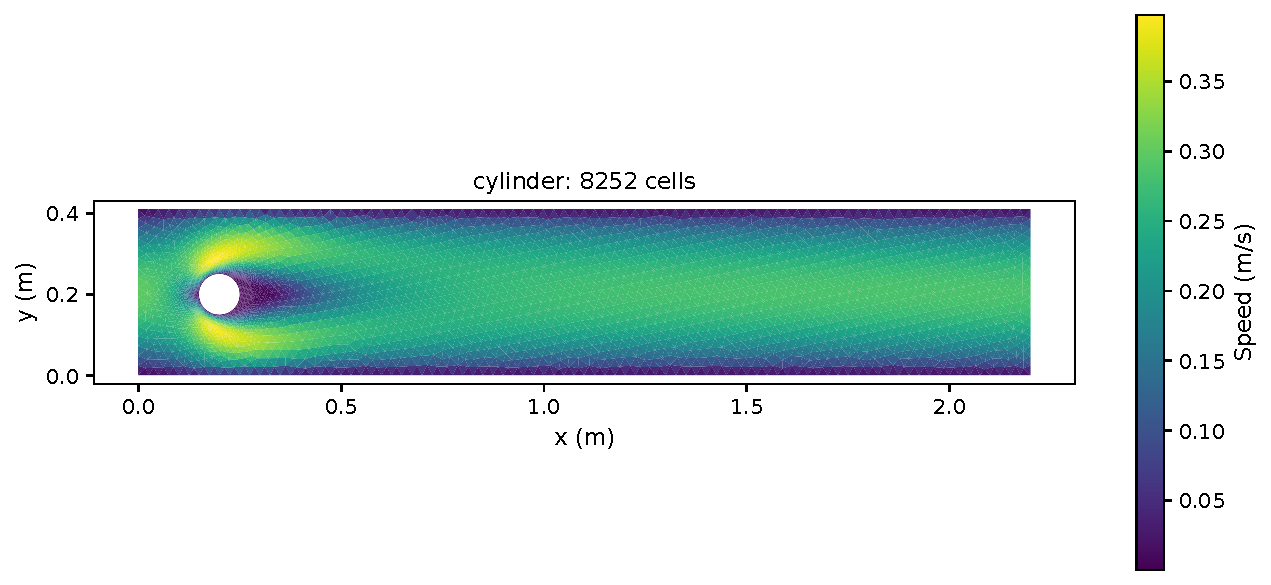
\includegraphics[width=.95\linewidth]{upwind/figures/velocity-global.pdf}\caption{upwind figures velocity global}\end{figure}\begin{figure}[p]\centering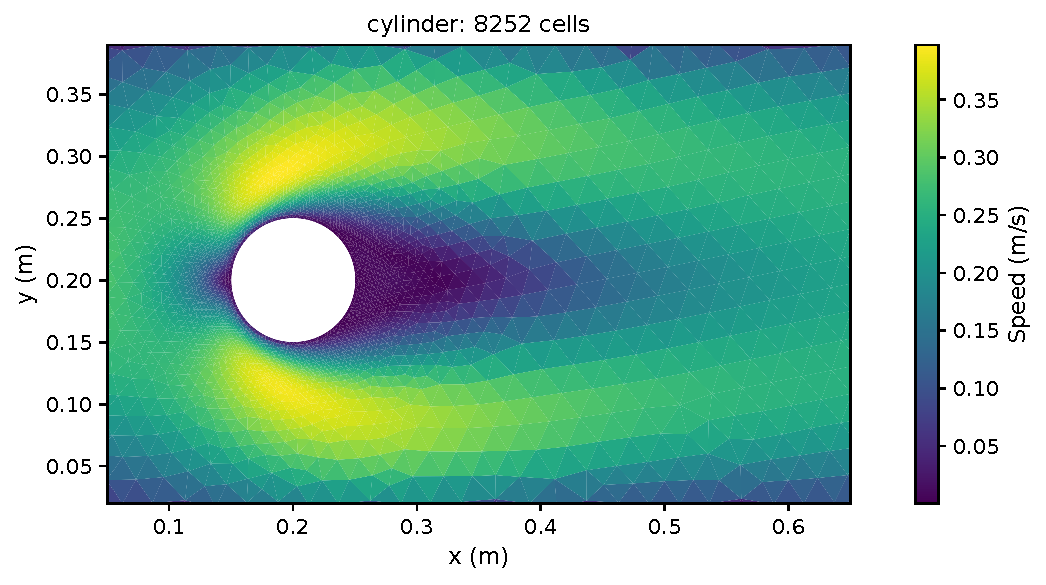
\includegraphics[width=.95\linewidth]{upwind/figures/velocity-local.pdf}\caption{upwind figures velocity local}\end{figure}\begin{figure}[p]\centering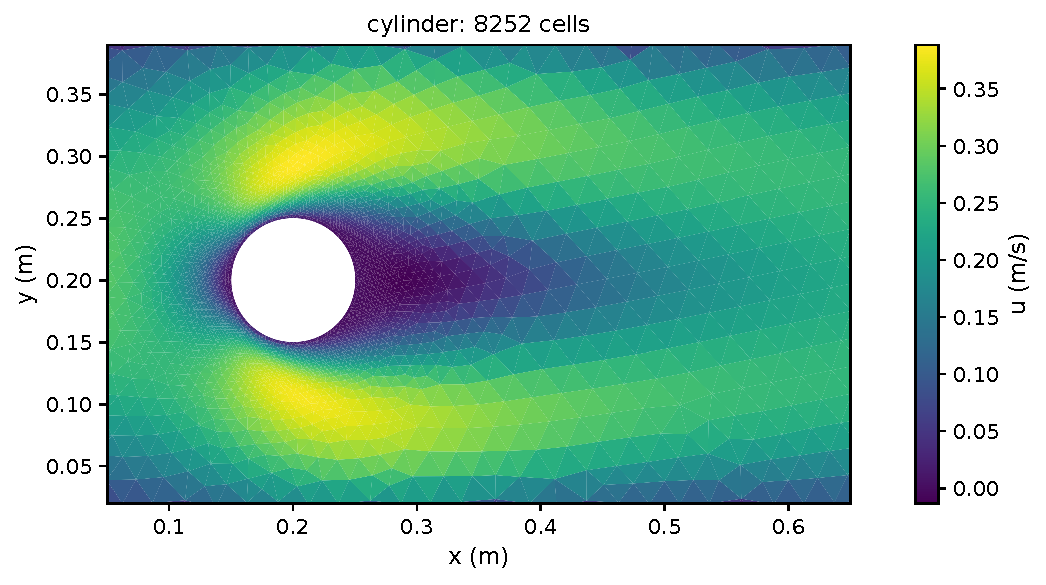
\includegraphics[width=.95\linewidth]{upwind/figures/u-local.pdf}\caption{upwind figures u local}\end{figure}\begin{figure}[p]\centering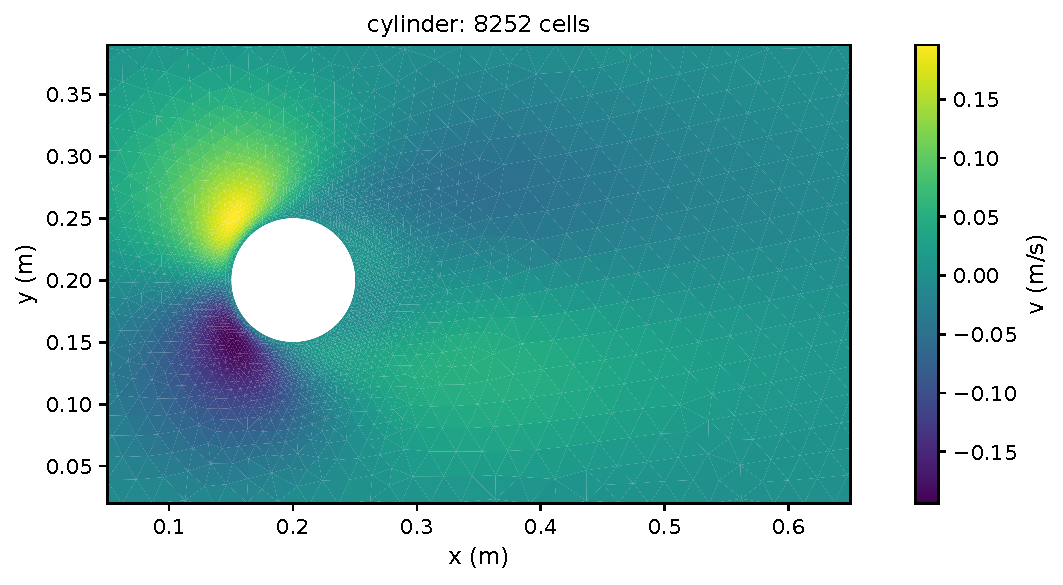
\includegraphics[width=.95\linewidth]{upwind/figures/v-local.pdf}\caption{upwind figures v local}\end{figure}\begin{figure}[p]\centering\includegraphics[width=.95\linewidth]{upwind/figures/mesh-local.pdf}\caption{upwind figures mesh local}\end{figure}\begin{figure}[p]\centering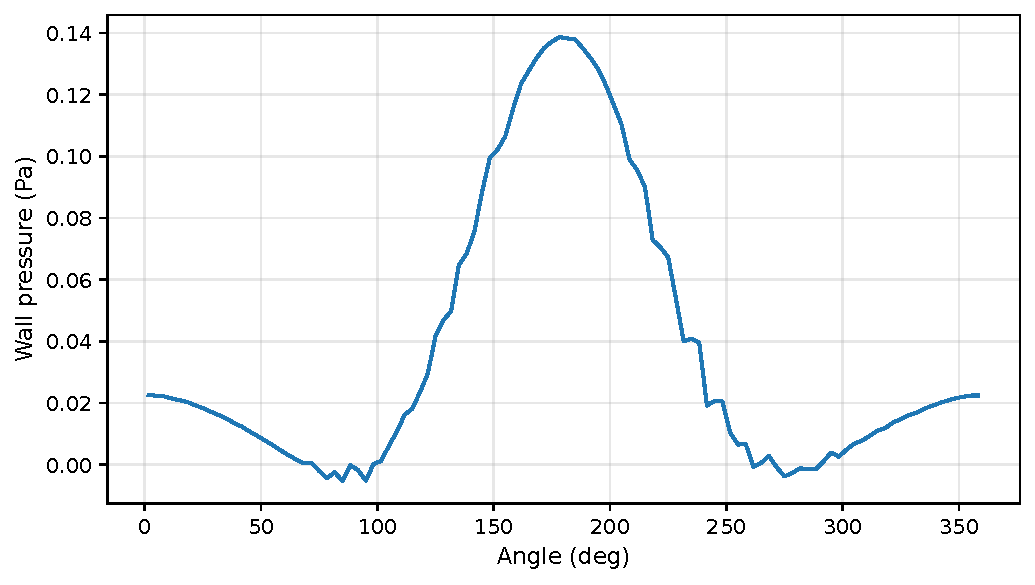
\includegraphics[width=.95\linewidth]{upwind/figures/surface-pressure.pdf}\caption{upwind figures surface pressure}\end{figure}\begin{figure}[p]\centering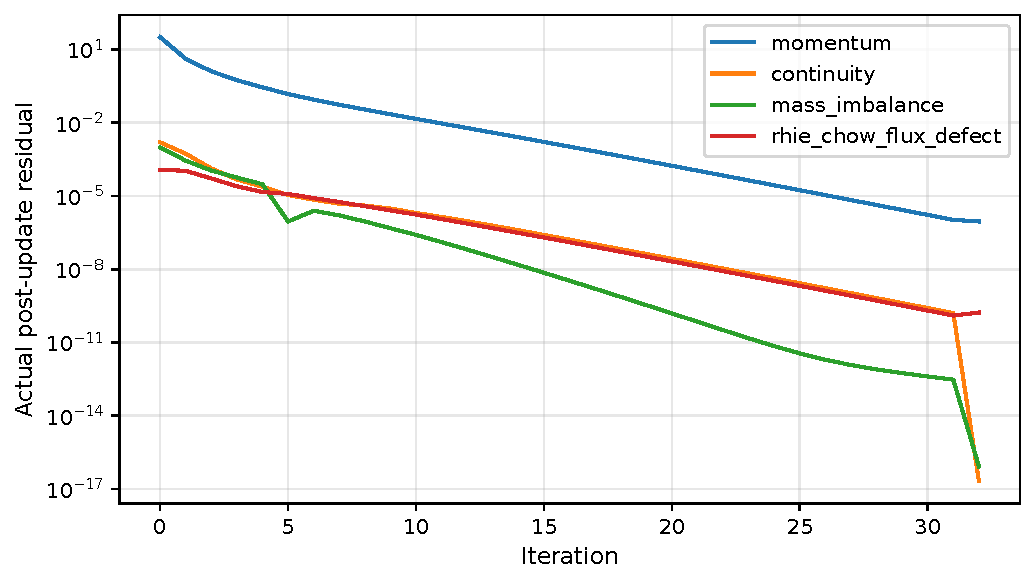
\includegraphics[width=.95\linewidth]{upwind/figures/residuals.pdf}\caption{upwind figures residuals}\end{figure}\begin{figure}[p]\centering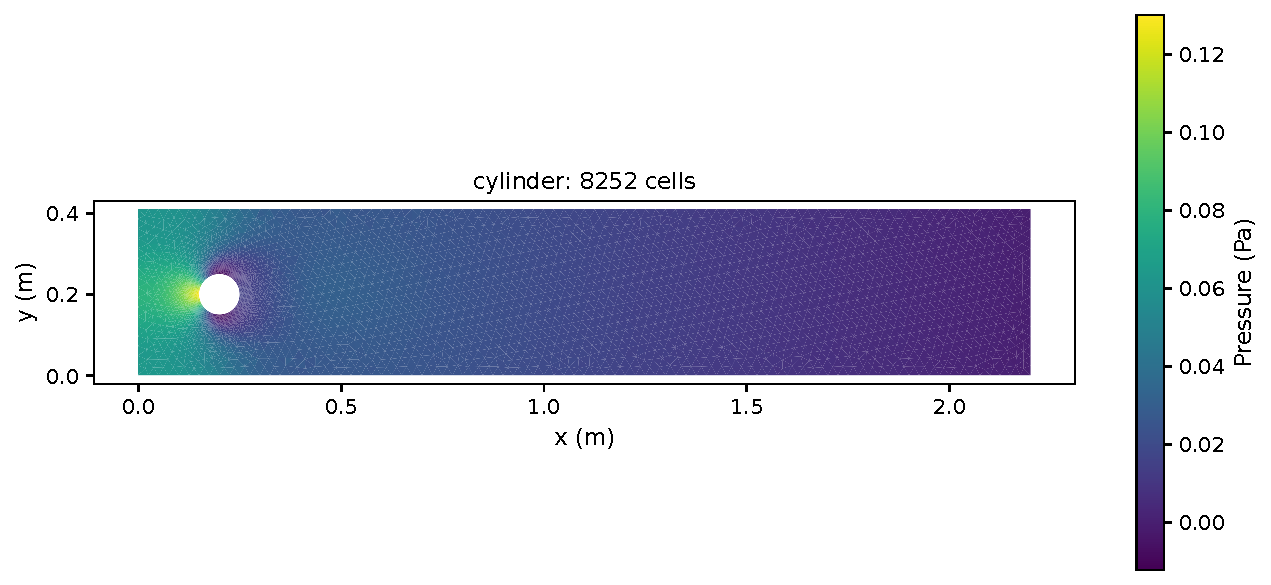
\includegraphics[width=.95\linewidth]{linear-upwind/figures/pressure-global.pdf}\caption{linear upwind figures pressure global}\end{figure}\begin{figure}[p]\centering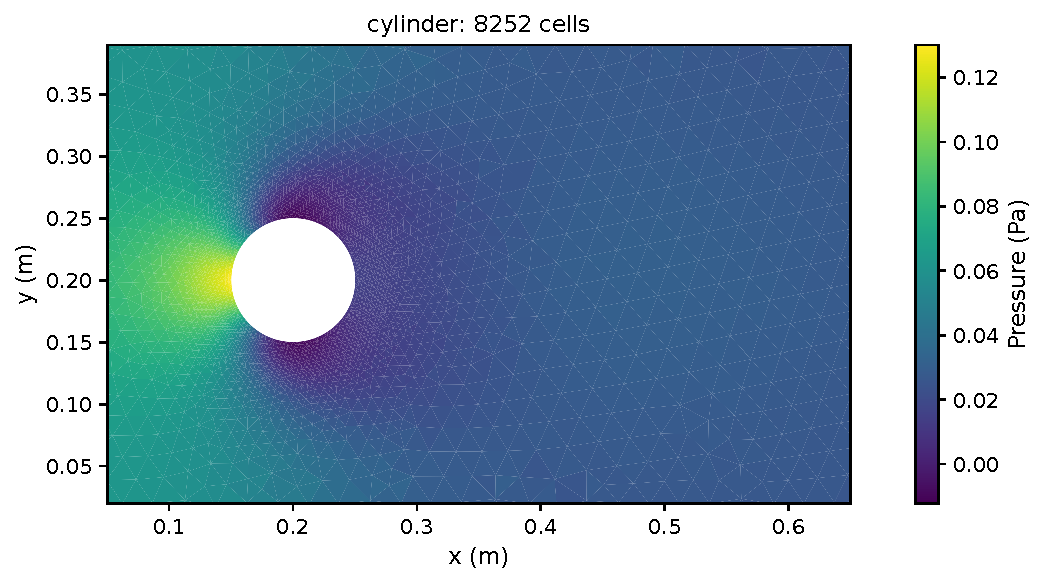
\includegraphics[width=.95\linewidth]{linear-upwind/figures/pressure-local.pdf}\caption{linear upwind figures pressure local}\end{figure}\begin{figure}[p]\centering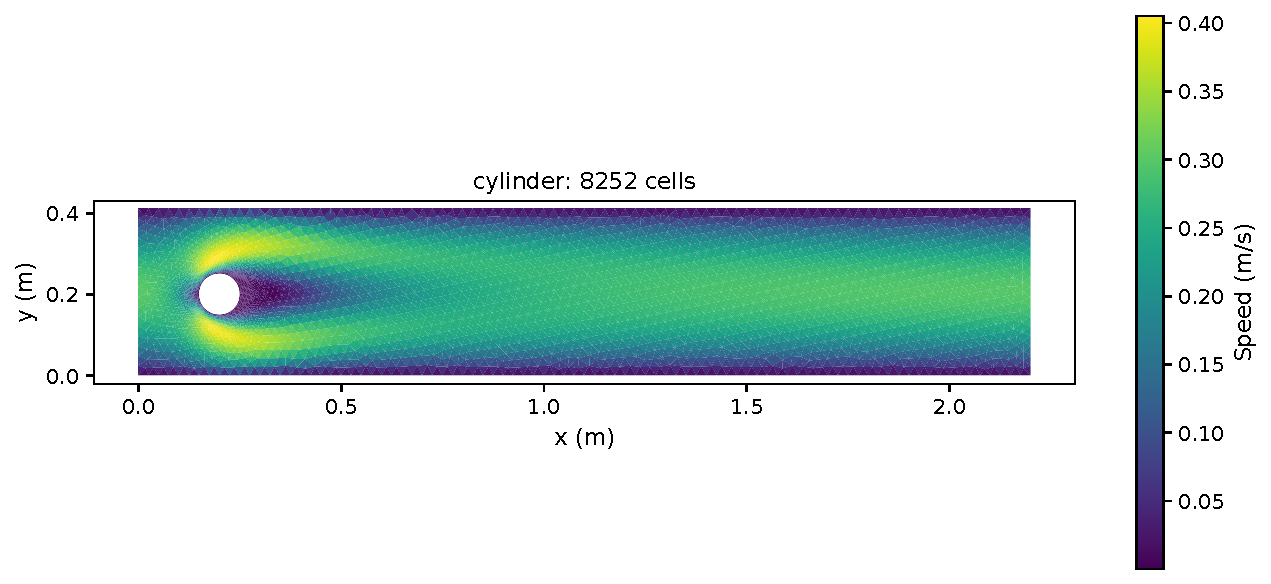
\includegraphics[width=.95\linewidth]{linear-upwind/figures/velocity-global.pdf}\caption{linear upwind figures velocity global}\end{figure}\begin{figure}[p]\centering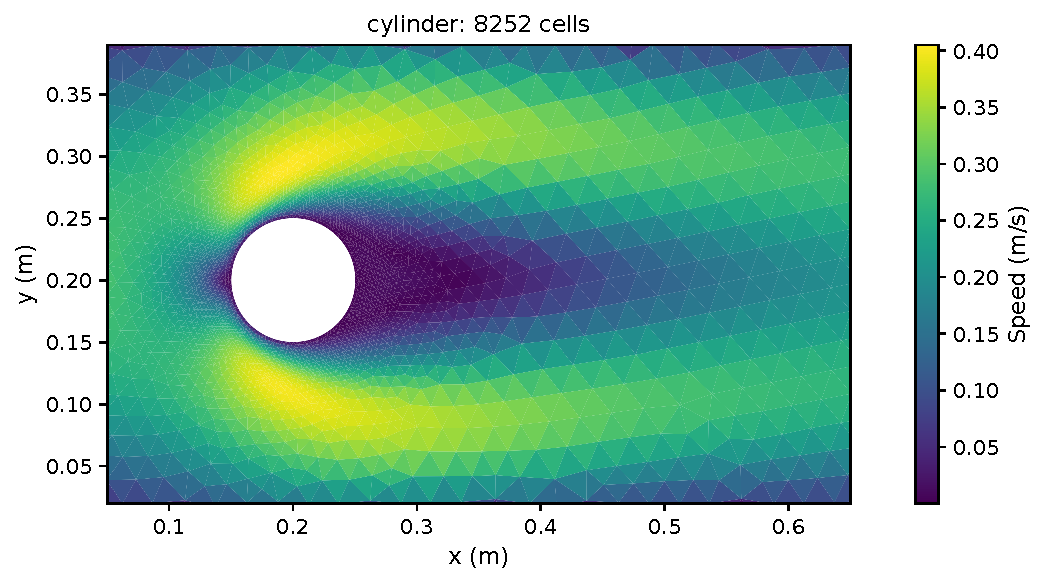
\includegraphics[width=.95\linewidth]{linear-upwind/figures/velocity-local.pdf}\caption{linear upwind figures velocity local}\end{figure}\begin{figure}[p]\centering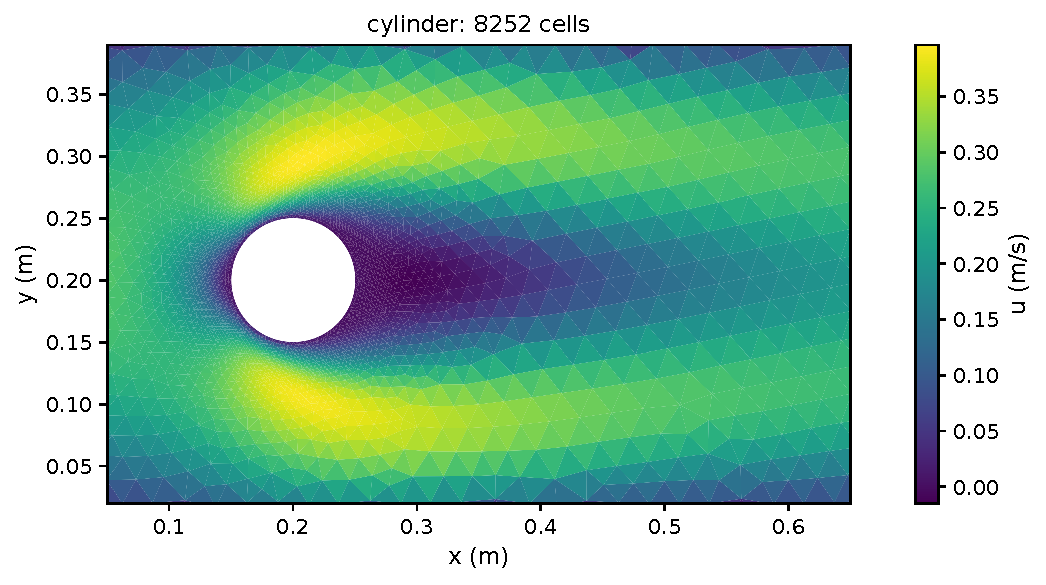
\includegraphics[width=.95\linewidth]{linear-upwind/figures/u-local.pdf}\caption{linear upwind figures u local}\end{figure}\begin{figure}[p]\centering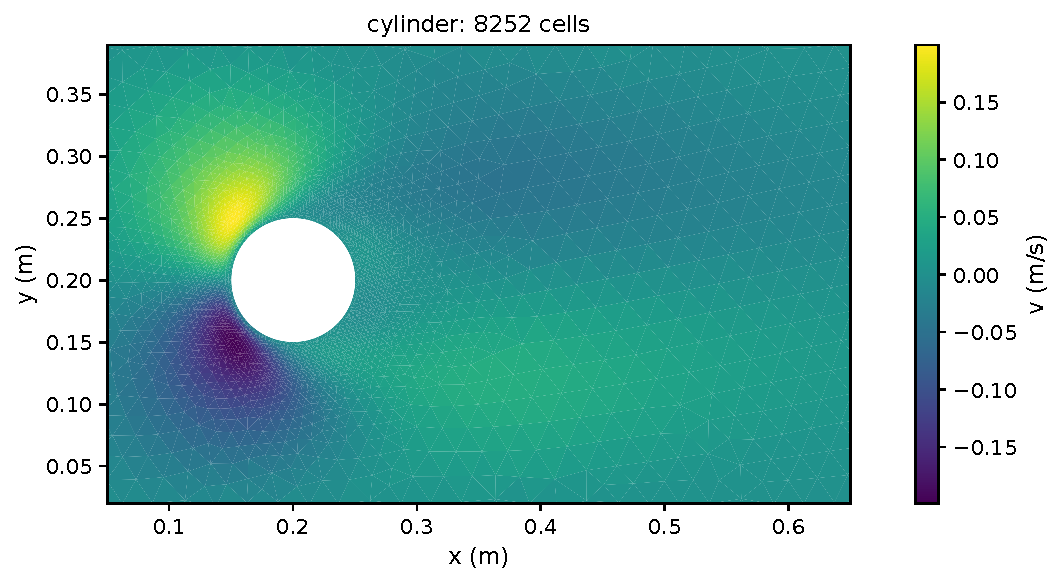
\includegraphics[width=.95\linewidth]{linear-upwind/figures/v-local.pdf}\caption{linear upwind figures v local}\end{figure}\begin{figure}[p]\centering\includegraphics[width=.95\linewidth]{linear-upwind/figures/mesh-local.pdf}\caption{linear upwind figures mesh local}\end{figure}\begin{figure}[p]\centering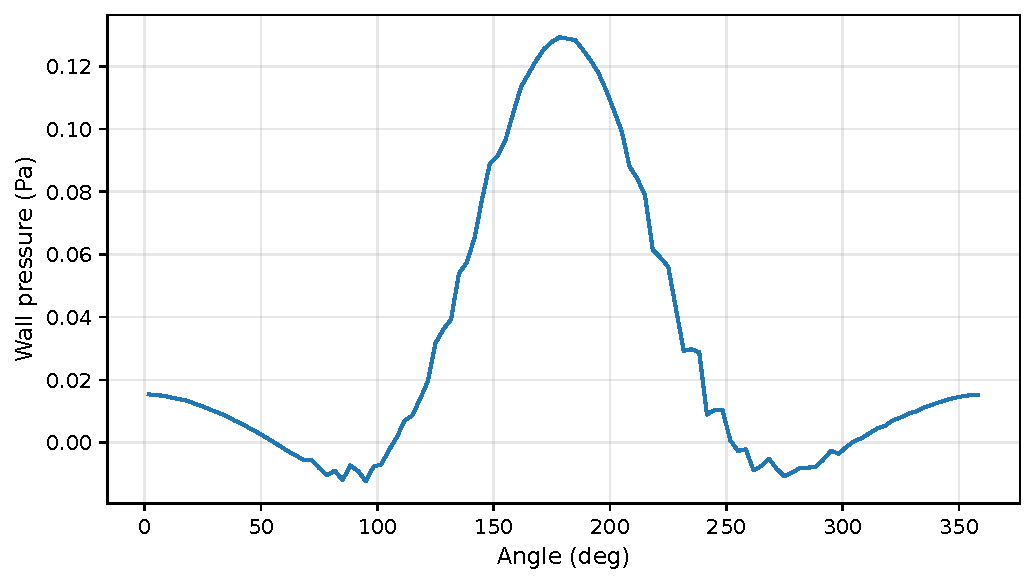
\includegraphics[width=.95\linewidth]{linear-upwind/figures/surface-pressure.pdf}\caption{linear upwind figures surface pressure}\end{figure}\begin{figure}[p]\centering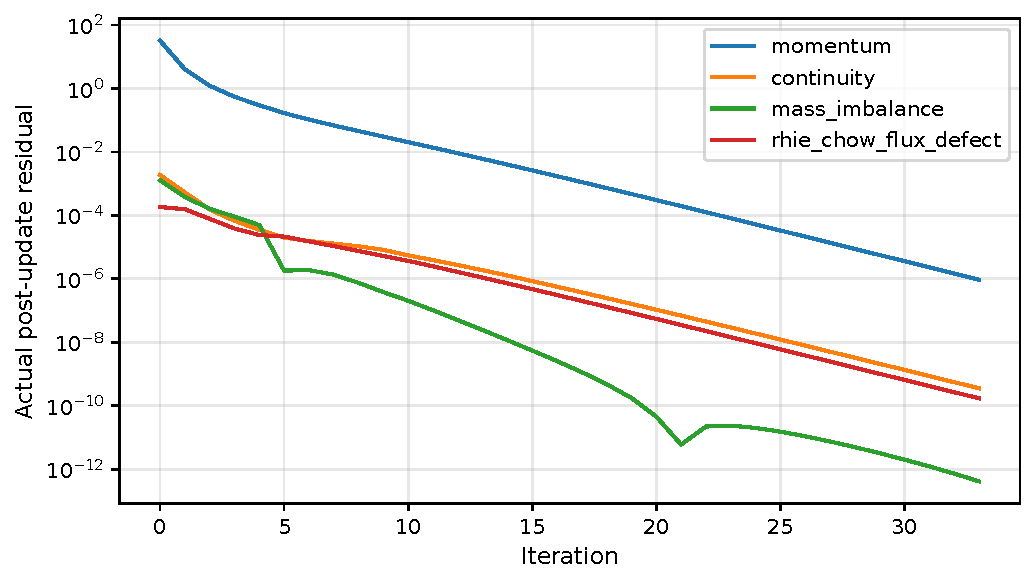
\includegraphics[width=.95\linewidth]{linear-upwind/figures/residuals.pdf}\caption{linear upwind figures residuals}\end{figure}\begin{figure}[p]\centering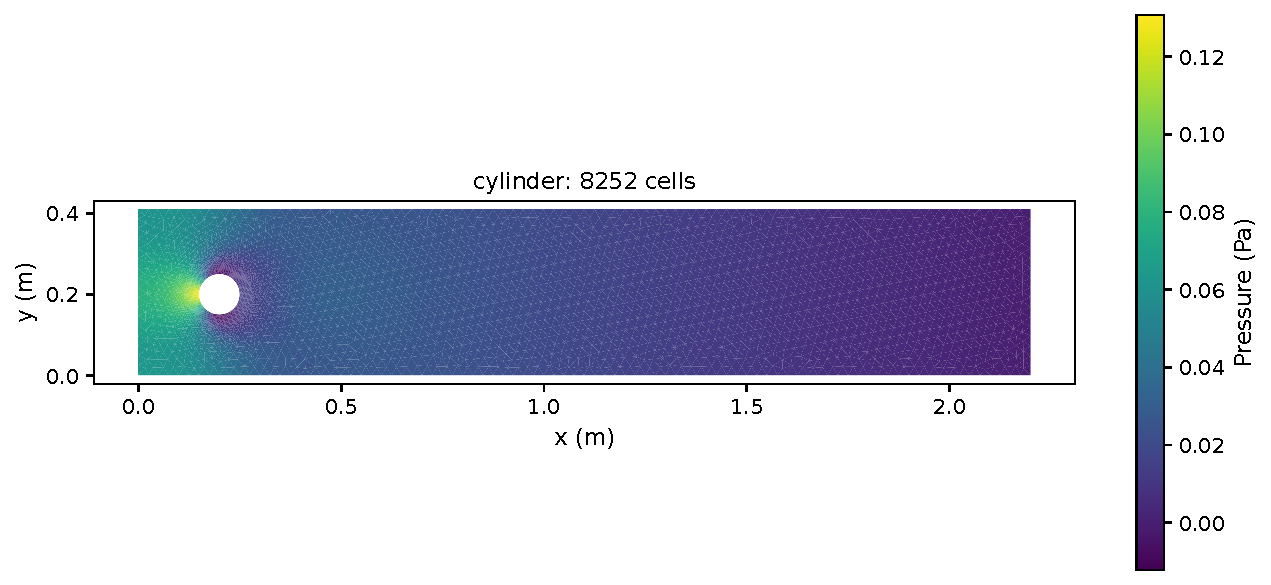
\includegraphics[width=.95\linewidth]{conservative-linear-upwind/figures/pressure-global.pdf}\caption{conservative linear upwind figures pressure global}\end{figure}\begin{figure}[p]\centering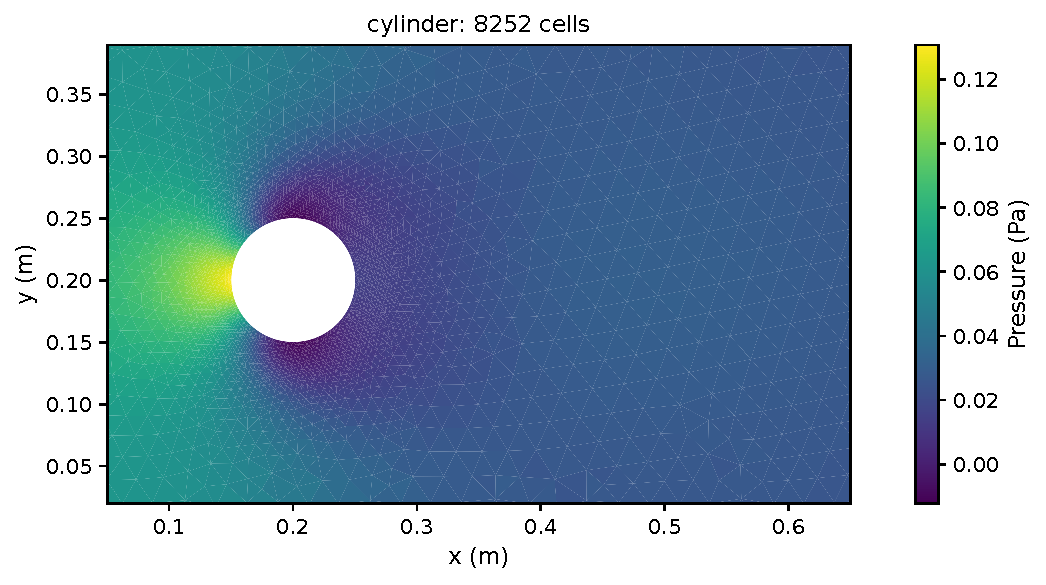
\includegraphics[width=.95\linewidth]{conservative-linear-upwind/figures/pressure-local.pdf}\caption{conservative linear upwind figures pressure local}\end{figure}\begin{figure}[p]\centering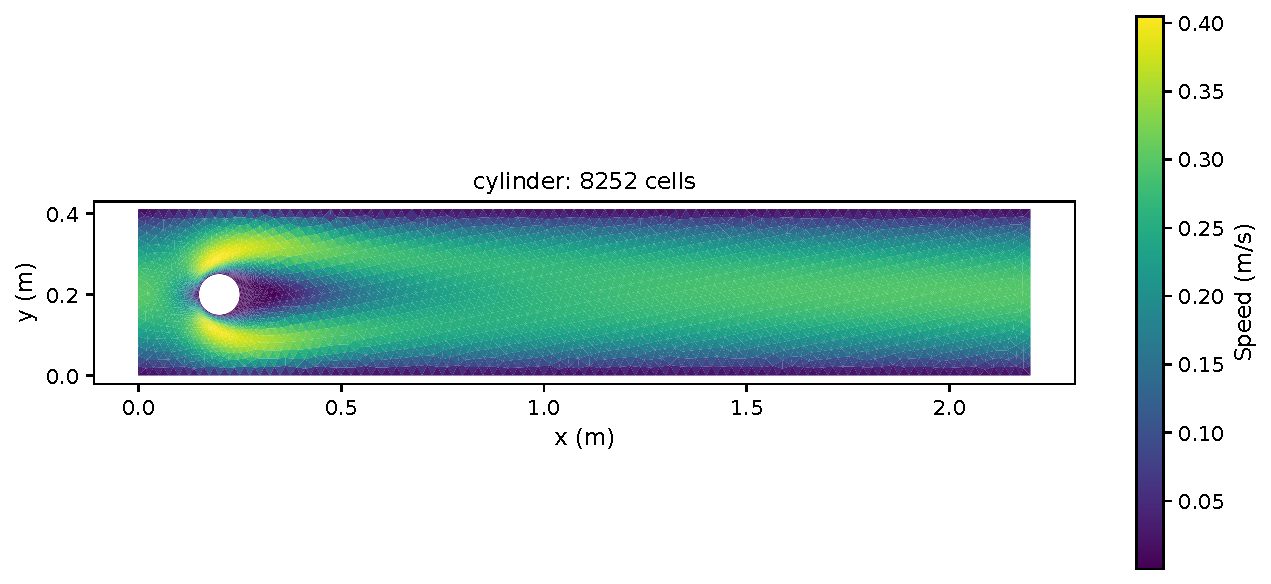
\includegraphics[width=.95\linewidth]{conservative-linear-upwind/figures/velocity-global.pdf}\caption{conservative linear upwind figures velocity global}\end{figure}\begin{figure}[p]\centering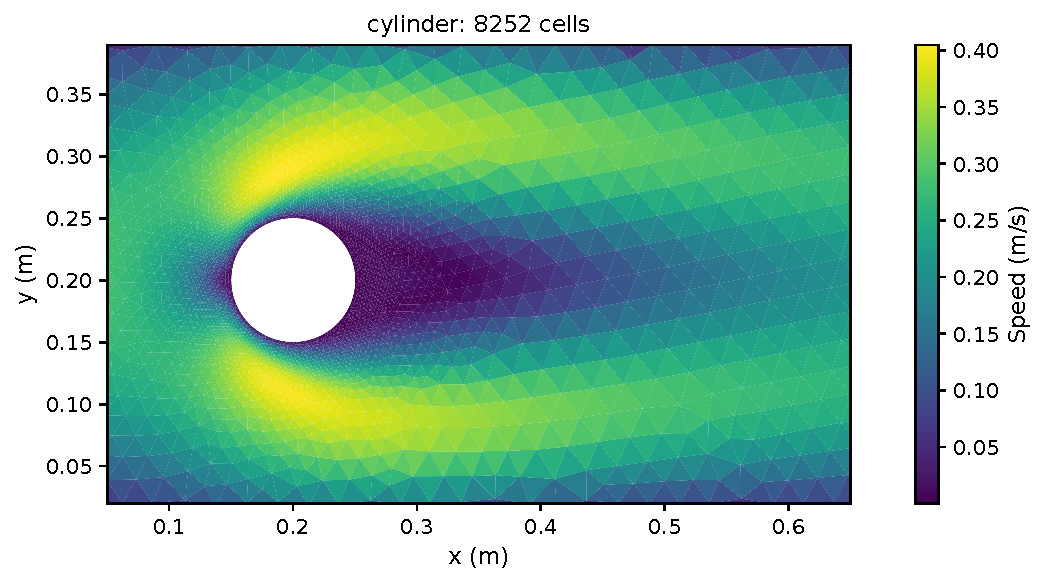
\includegraphics[width=.95\linewidth]{conservative-linear-upwind/figures/velocity-local.pdf}\caption{conservative linear upwind figures velocity local}\end{figure}\begin{figure}[p]\centering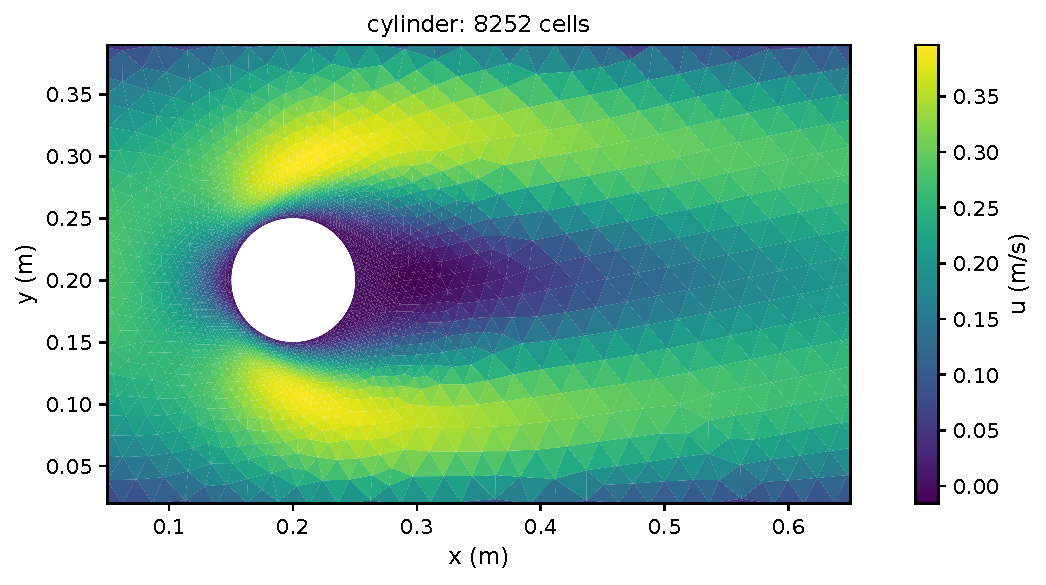
\includegraphics[width=.95\linewidth]{conservative-linear-upwind/figures/u-local.pdf}\caption{conservative linear upwind figures u local}\end{figure}\begin{figure}[p]\centering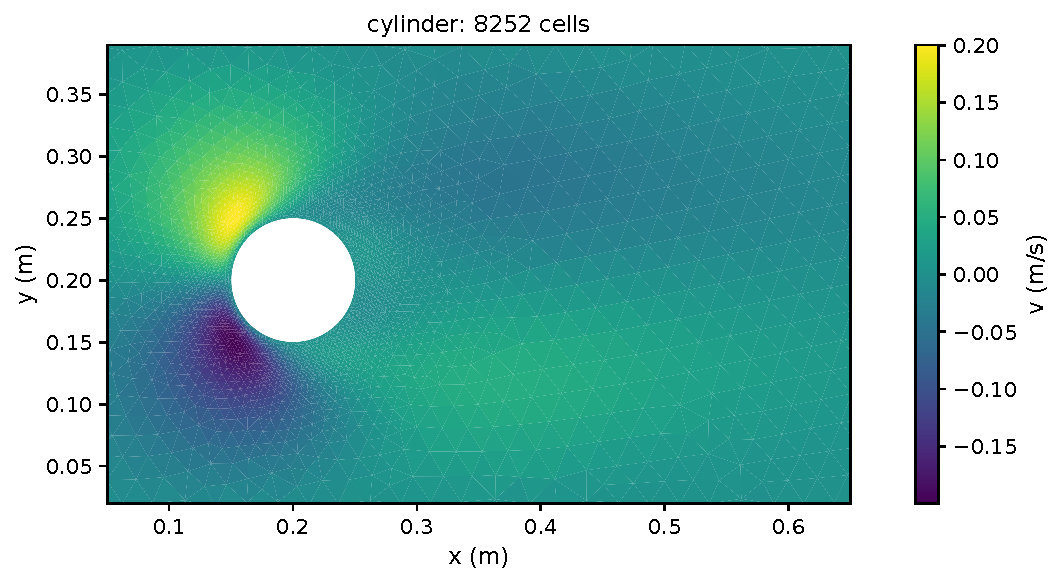
\includegraphics[width=.95\linewidth]{conservative-linear-upwind/figures/v-local.pdf}\caption{conservative linear upwind figures v local}\end{figure}\begin{figure}[p]\centering\includegraphics[width=.95\linewidth]{conservative-linear-upwind/figures/mesh-local.pdf}\caption{conservative linear upwind figures mesh local}\end{figure}\begin{figure}[p]\centering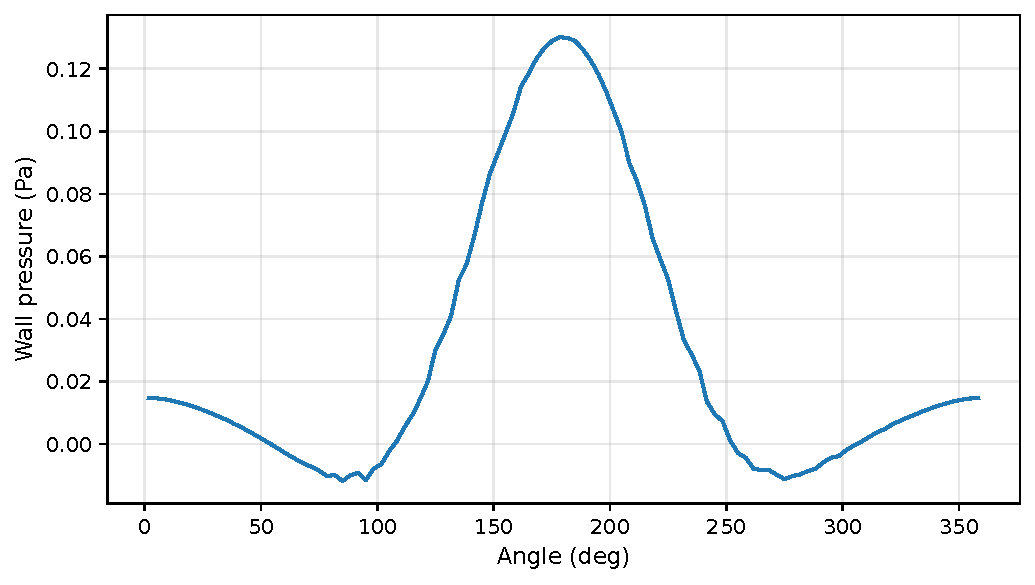
\includegraphics[width=.95\linewidth]{conservative-linear-upwind/figures/surface-pressure.pdf}\caption{conservative linear upwind figures surface pressure}\end{figure}\begin{figure}[p]\centering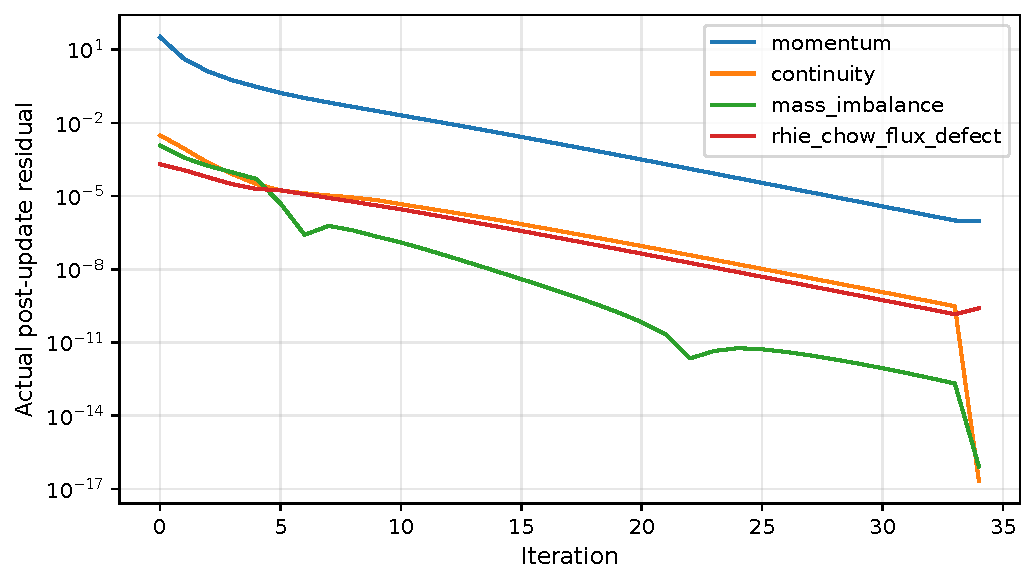
\includegraphics[width=.95\linewidth]{conservative-linear-upwind/figures/residuals.pdf}\caption{conservative linear upwind figures residuals}\end{figure}\begin{figure}[p]\centering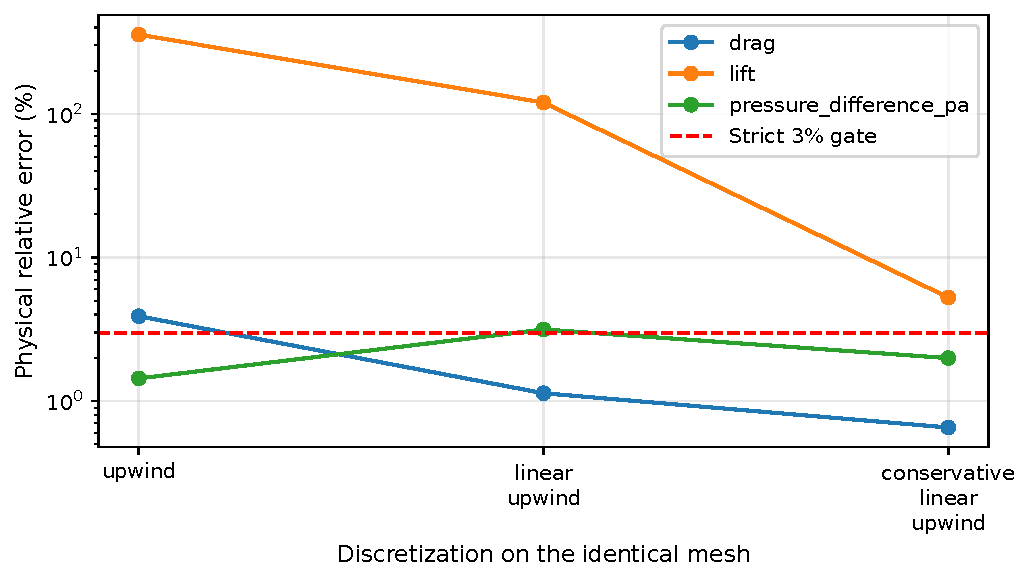
\includegraphics[width=.95\linewidth]{refinement.pdf}\caption{refinement}\end{figure}\end{document}
